\documentclass[11pt, oneside]{article}   	% use "amsart" instead of "article" for AMSLaTeX format
\usepackage{geometry}                		% See geometry.pdf to learn the layout options. There are lots.
\geometry{letterpaper}                   		% ... or a4paper or a5paper or ... 
%\geometry{landscape}                		% Activate for rotated page geometry
%\usepackage[parfill]{parskip}    		% Activate to begin paragraphs with an empty line rather than an indent
\usepackage{graphicx}				% Use pdf, png, jpg, or eps§ with pdflatex; use eps in DVI mode
								% TeX will automatically convert eps --> pdf in pdflatex		
\usepackage{amssymb}

\usepackage{geometry}

\usepackage{hyperref}
\hypersetup{
colorlinks=true,
linkcolor=blue,
}

\usepackage{fancyhdr}
\pagestyle{fancy}

\graphicspath{{./Gantt/}}

\lhead{Mehta, Jash
		- mehtaj8\\
		Sharma, Aditya
		- shara24\\
		Ren, Zackary
		- renx11}
\chead{SE 3XA3 DP-Rev0}
\rhead{\today}

\title{Development Plan}
\author{}
%\date{}							% Activate to display a given date or no date
%\begin{header}

%\end{header}
\begin{document}
%\maketitle
\newgeometry{headsep = {50pt}}
\section*{Development Plan}
\subsection*{Team Meeting Plan}
\subsubsection*{Pre-Development}
\begin{enumerate}

\item Meet every lab-session to work on the assignments \& milestones.
\item Lead Developer to provide progress reports/summaries at the end of each lab.
\item Lead Developer to provide tasks/a plan-of-action for each item the team has to accomplish by the next lab session. 
\item Meeting Agenda will have the following information to be filled in during each meeting.

\begin{enumerate}
\item Previous Agenda items.
\begin{enumerate}
\item Will go through Agenda items from last meeting to see what work is in progress and how much progress has been made.
\end{enumerate}

\item List of topics for current week.
\begin{enumerate}
\item Will have Decision section for each topic.
\end{enumerate}

\item Work plan for each developer for the week (Homework).
\end{enumerate}

\end{enumerate}

\subsubsection*{Development}
\begin{enumerate}
\item Hold stand-up meetings every 2 days discussing our progress
\item Lead Developer to provide daily progress reports/summaries
\item Meet during lab sessions to discuss blocking issues and debug
\item Meeting Agenda will have the following information to be filled in during each meeting.

\begin{enumerate}
\item Previous Agenda items.
\begin{enumerate}
\item Will go through Agenda items from last meeting to see what work is in progress and how much progress has been made.
\end{enumerate}

\item List of topics for current week.
\begin{enumerate}
\item Will have Decision section for each topic.
\end{enumerate}

\item Work plan for each developer for the week (Homework).
\end{enumerate}
\end{enumerate}

\newgeometry{headsep = {50pt}}
\newpage
\subsection*{Team Communication Plan}
\subsubsection*{Pre-Development}
\begin{enumerate}
\item Communication during this period is to be done through a combination of Microsoft Teams and Facebook Messenger.
\item Teams is to be used as a way to provide weekly updates on progress, upcoming tasks, questions and concerns, and as well as possible issues.
\item Messenger will be used as a way to communicate on a daily basis in terms of providing a way to answer simple questions and track progress on tasks when closer to deadline.
\end{enumerate}

\subsubsection*{Development}
\begin{enumerate}
\item All communication shall be done over Teams during Development
\item Weekly updates shall be provided by the Lead Developer to the Team via Microsoft Teams. These updates shall encompass the following (progress summary, upcoming tasks, possible challenges). If there are any issues or any unpredicted set-backs, the update shall also include the following: brief plan of attack, revised plans, updated time-line.
\item Milestones shall be tracked via the \href{https://gitlab.cas.mcmaster.ca/renx11/3xa3-project-l02-group9/-/boards}{Kanban Board} on GitLab.
\end{enumerate}


\newgeometry{headsep = {50pt}}
\newpage
\subsection*{Team Member Roles}
\begin{tabular}{ | c | c | c |}
\hline
Name & Role & Expertise \\
\hline
Aditya Sharma & Developer, QA & React, Node, Python, TS/JS, Git, Latex\\
\hline
Jash Mehta & Lead Developer, QA & React, Node, Python, TS/JS, Git, Latex\\
\hline
Zackary Ren & Developer, QA & React, Node, Python, TS/JS, Git, Latex\\
\hline
\end{tabular}
\\
\begin{itemize}
\item The Lead Developer will handle daily/weekly reports and keep track of progress using the meeting agenda and Gantt chart. Developer responsibilities are encompassed as well.\\

\item The Developer is responsible for creating the features assigned to them and resolving the bugs involved with their feature. Features are assigned based on the SRS created by the team.\\

\item The QAs' (Quality Assurance) is responsible for creating test cases relevant to the feature they are assigned to. This is to ensure that the feature adheres to the correct specification.\\
\end{itemize}

\newgeometry{headsep = {50pt}}
\newpage
\subsection*{Git Workflow Plan}

Our Git Workflow shall revolve around the simplified version of the Gitflow Workflow practice. Throughout the development process of the project, we will be leveraging 2 different branches: {\it master} and {\it development}. The {\it master-branch} will store the official release of the project, whereas the {\it develop-branch} will be the integration branch for all the features/tickets.\\

We will also be leveraging the concept of a {\it feature-branch}. Each feature/ticket shall be implemented within a {\it feature-branch} whose respective parent is the {\it develop-branch}. This ensures that when the development and testing process for a feature is complete, it can be merged with the {\it develop-branch} rather than the {\it master-branch}.\\ 

Our project will not be leveraging {\it release} or {\it hotfix} branches due to the intended small scale and simplicity of the project. We feel that by adding these branches, we would overcomplicate the production, testing and release of our software.\\

\newgeometry{headsep = {50pt}}
\newpage
\subsection*{Proof of Concept Demonstration Plan}  

The most significant risk would be a lack of consistency amongst the developers' work environments. Inconsistencies in software library versions could introduce unnecessarily complicated bugs. We will ensure that all developers’ environments are set up the same way to avoid the aforementioned issue.\\

We believe that unit testing will not be difficult because we have significant experience with unit testing via 2AA4 and 2XB3. However, we believe that integration testing presents certain challenges. This is because we have to mock the API and front-end interactions to simulate different kinds of interactions the end user would have with our app.\\

The most common roadblock in team-oriented software development is setting up the development environment and tools. The development environment and tools that are being used across everybody's machine needs to be consistent otherwise there is a risk of producing bugs later in the development period that are difficult to resolve.
The second part of implementation that might be difficult will be deploying the front-end and back-end. This is because we will be using technologies that we have little hand-on experience with. However, we hope to overcome this burden by focusing all of our attention on 1 task at a time (backend first, then frontend). This ensures that everybody is aware of what is happening in the software and in the event that a bug rises, multiple developers are capable of contributing to its resolution rather than just the developer who made the feature.\\

There are no libraries that are particularly difficult to install. However, this does not mean that the libraries will be easy to use because we do not have experience with some of them (Flask). By the same token, we plan on leveraging existing documentation and publicly available resources (udemy, stackoverflow and github issues) to ensure that we understand the library and overcome any issues that arise from its use within an appropriate timeframe.\\

Portability will always be a concern with any software product. However, we plan on ensuring that our software product is portable via the choice of the technologies that we are using. By using React-Native, we are able to cater to customers in both iOS and Android markets. Furthermore, by leveraging Docker, we are able to containerize the application and ensure that it can be run from any environment for development. This significantly improves portability of the software product after release and during development as well.\\

\newgeometry{headsep = {50pt}}
\newpage
\subsection*{Technology}

\begin{itemize}
\item \it React-Native
\item \it Python - Beautiful-Soup, Selenium\ \&\ Flask
\item \it Prettier - ESLint, Bracket Colorizer
\item \it Docker
\end{itemize}

As mentioned in the Project Statement, our software product is a mobile application intended for both iOS and Android devices. As a result, we need to leverage a technology that will enable us to produce and deliver a high quality product for both mobile environments. \\

Normally, in order to produce a product for an iOS and Android device, we would need to leverage {\it Swift} and {\it Java} respectively. This would result in either 2 separate code-bases or 1 massive code-base. This would introduce an extra-layer of complexity to the project. Therefore, we have decided to use a cross-platform technology known as {\it React-Native}. This programming language/framework will allow us to develop for both platforms through a singular codebase. \\

We will also be leveraging {\it Beautiful-Soup} \& {\it Selenium} to perform the web-scraping. The backend logic will be hosted by an API and this API will be created via {\it Flask}. \\

A CI/CD pipeline will be leveraged to automate builds, testing and deployments. We will be leveraging the built-in CI/CD pipelining support offered by GitLab. This requires the use of a Docker image which is why we will be using Docker. \\

\newgeometry{headsep = {50pt}}
\newpage
\subsection*{Coding Style}

A strict coding style shall be enforced for the purpose of readability, maintainability and quick iterations. This coding style shall be enforced via the use of tools such as {\it Prettier}, {\it ESLint} \& {\it Flake8}. These tools are plugins that can be installed onto our IDE ({\it VS Code}). These tools will handle things such as spacing, variable naming, maximum-line length etc…\\

To keep the project simple, we will not be using a state-management system such as {\it MobX} or {\it Redux}. Instead, we will be leveraging the built-in state-management tools offered by {\it React-Native}.

\subsubsection*{General Rules}
\begin{enumerate}
\item Keep things simple.
\item Find the root cause of bugs.
\item Put all boundary conditions in 1 place (don’t have different edge cases for multiple functions). Handle edge case processing in 1 place.
\item Descriptive, meaningful, unambiguous names.
\item No constants (all constants will be declared in a file in the root directory known as constants.extension).
\item Keep functions small - each function should only do 1 task.
\item Minimize the number of arguments to a function.
\item Add Brief comments on a function if the function name is not sufficient enough to describe it.
\item When testing, only have 1 assert per test and provide each test a meaningful description.
\end{enumerate}

\newgeometry{headsep = {50pt}}
\pagebreak
\subsubsection*{React-Native Rules}
\begin{enumerate}
\item We will be using Function Components. 
\item Interfaces will have a leading “I” prefacing the name of the variable. For example: “ITodoItem” will represent the interface for a “TodoItem”.
\item Props will always end with “Props”. For example: “TodoItemProps” will represent the props object being passed into the “TodoItem” component. 
\item Stylesheets pertaining to a particular component will always be located at the bottom of the page.
\end{enumerate}


\subsubsection*{Python Rules}
\begin{enumerate}
\item Following {\it Pep8} Style Guide, using {\it Flake8} as our automated linter.
\item Automatically updates coding style to fit {\it Pep8} guidelines, therefore the {\it Flake8} linter provides adherence.
\end{enumerate}

\newgeometry{headsep = {50pt}}
\newpage
\subsection*{Project Schedule}
\subsubsection*{Gantt Chart}
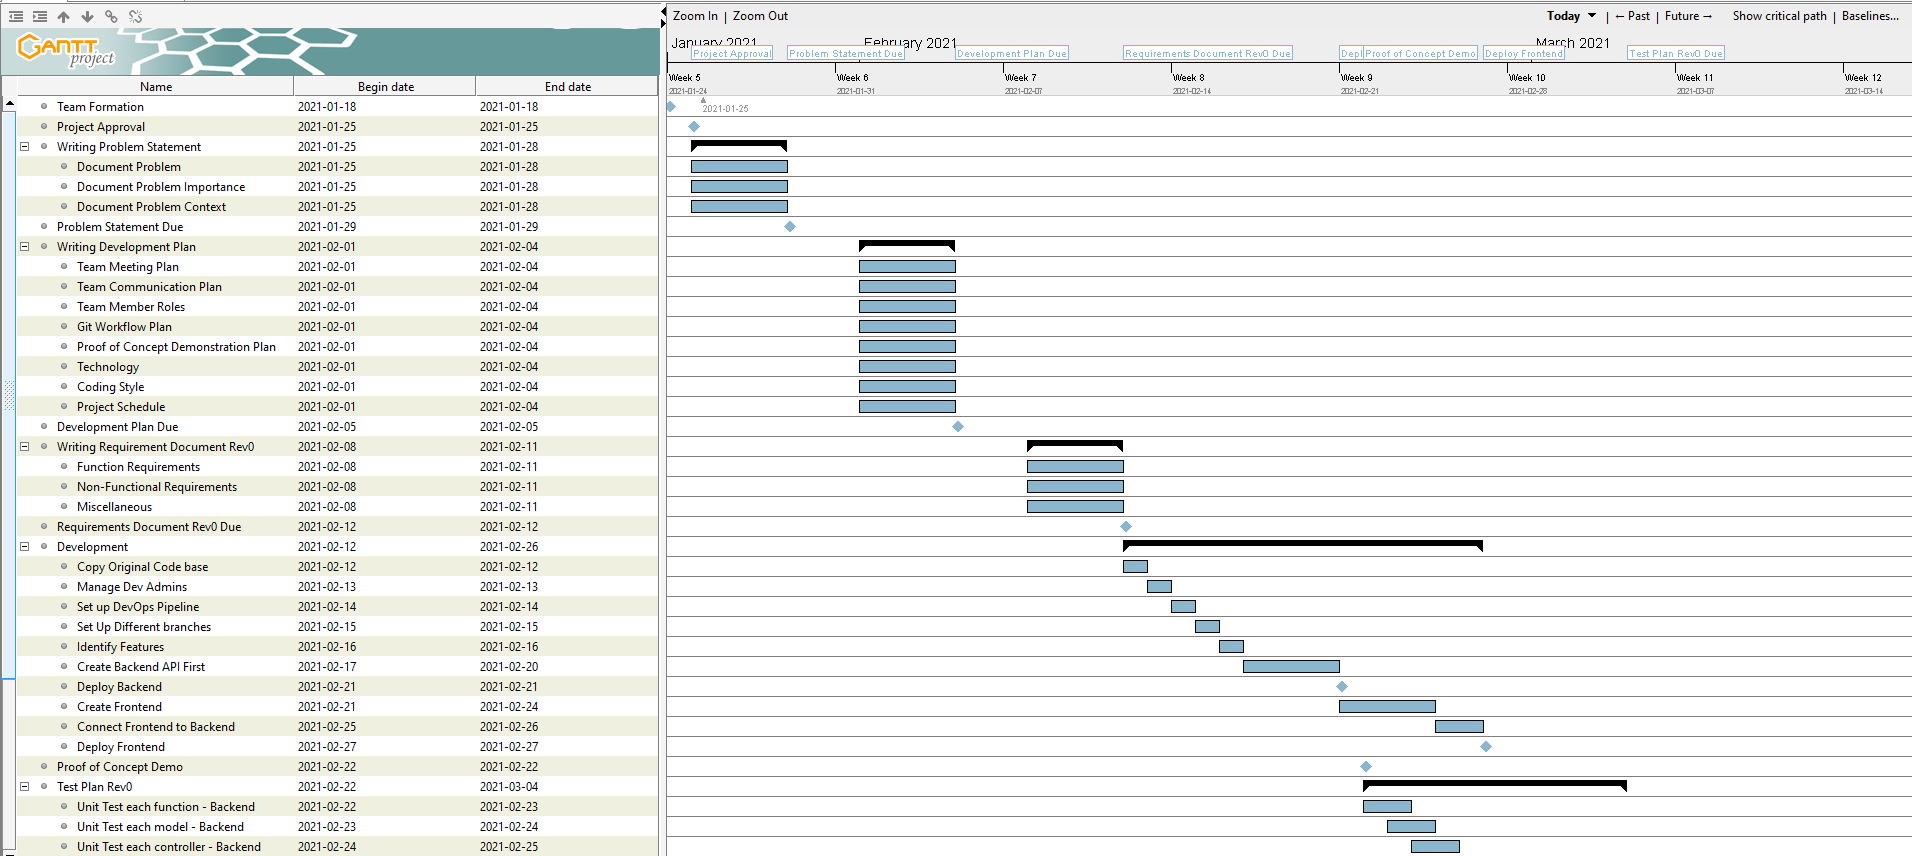
\includegraphics[scale=0.3]{Screenshot1}
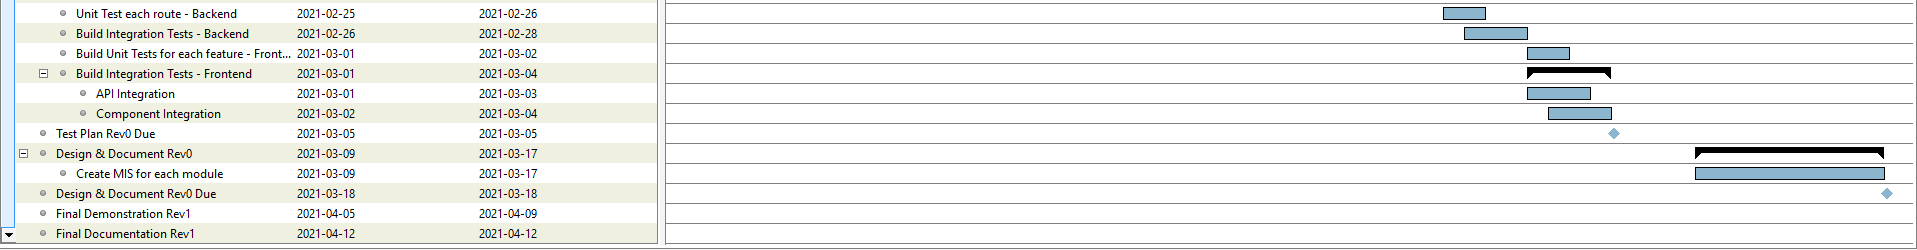
\includegraphics[scale=0.3]{Screenshot2}\\

\newgeometry{headsep = {50pt}}
\pagebreak
\noindent
\subsubsection*{Resource Allocation}
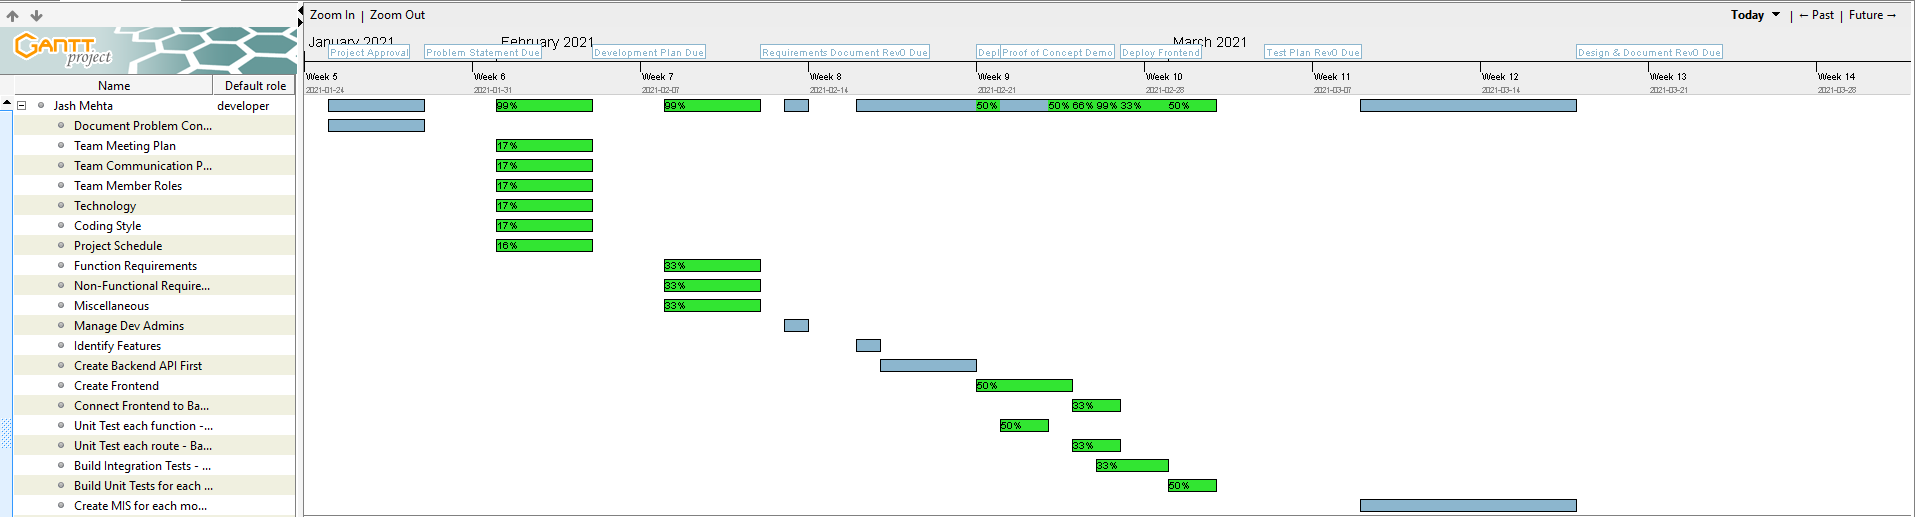
\includegraphics[scale=0.3]{Jash}
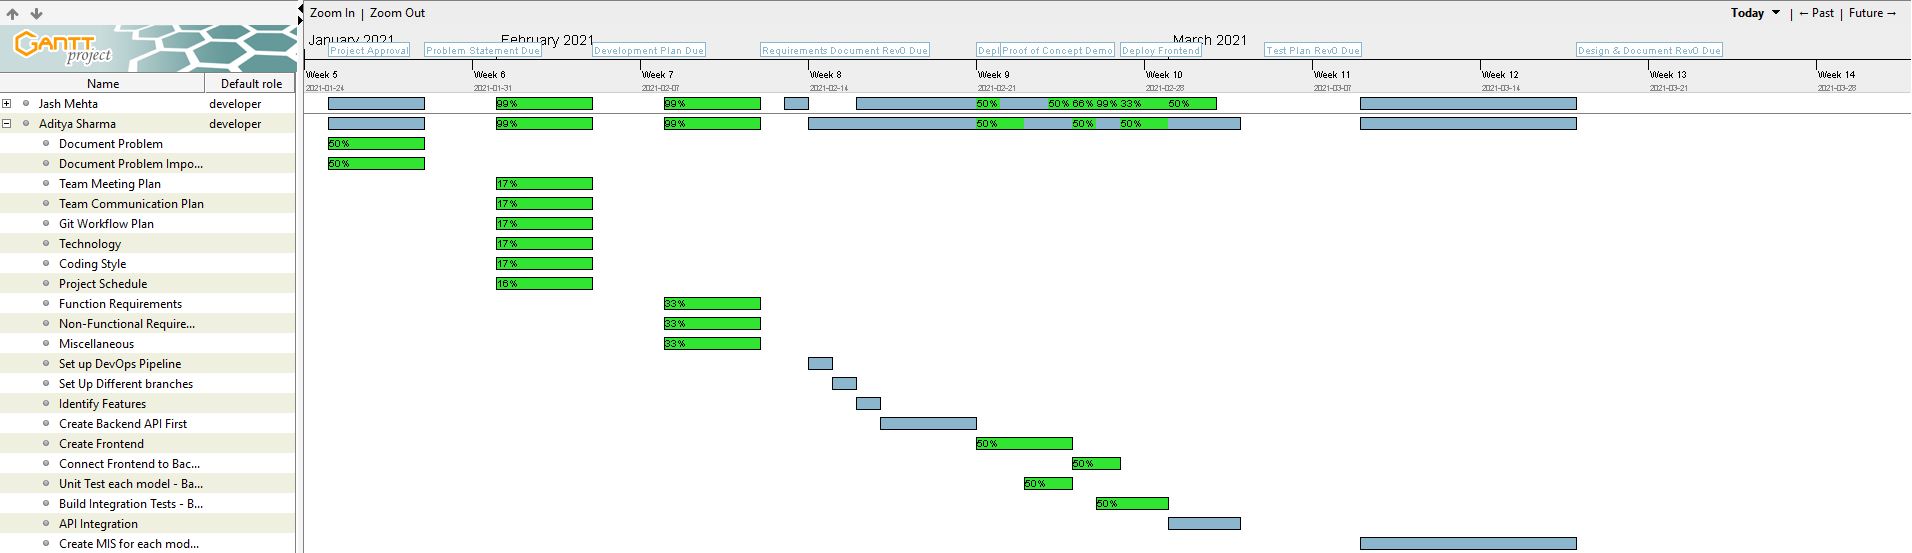
\includegraphics[scale=0.3]{Aditya}
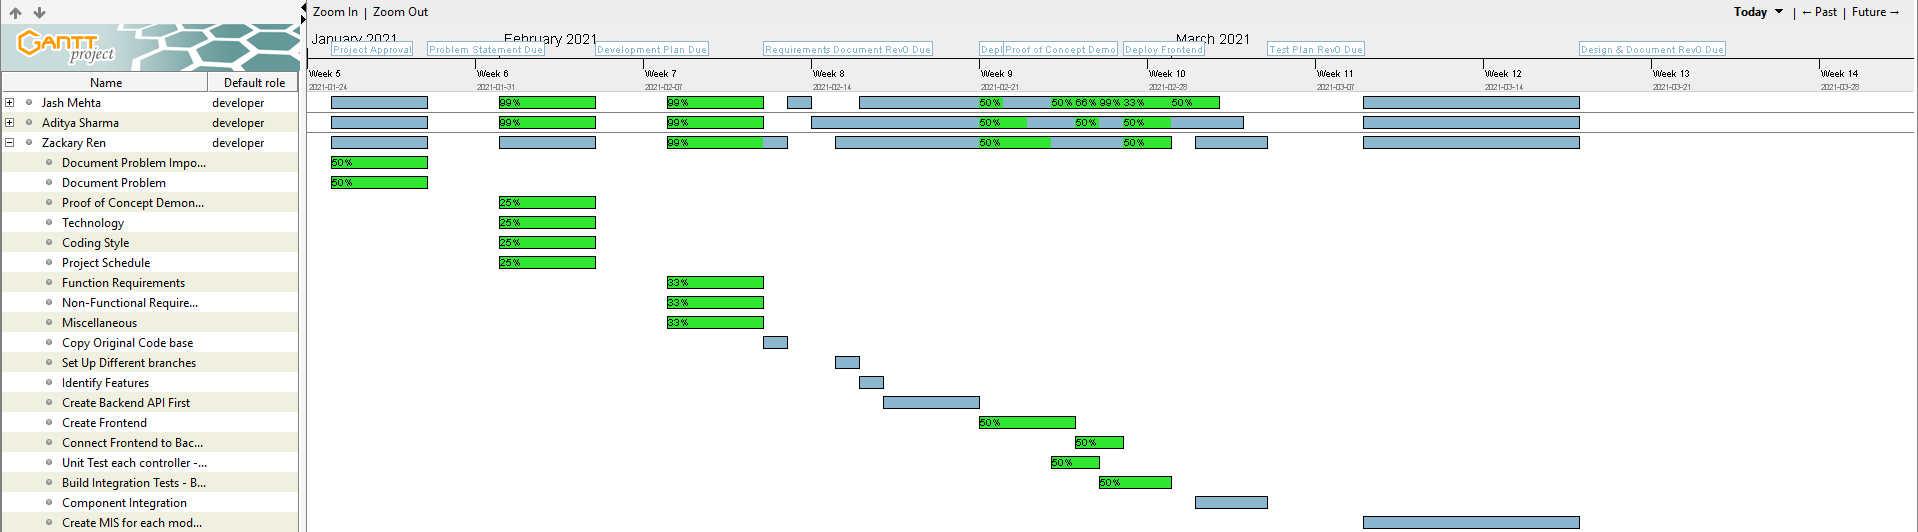
\includegraphics[scale=0.3]{Zackary}
\newgeometry{headsep = {50pt}}
\newpage
\subsection*{Project Review}
\end{document}  
